\documentclass[12pt, letterpaper, twoside]{article}

\usepackage[utf8]{inputenc}
\usepackage{listings}
\usepackage{color}
\usepackage{algorithm}
\usepackage{algpseudocode}
\usepackage{graphicx}
\usepackage{amsmath}
\usepackage{algpseudocode}
\usepackage{enumitem}

\graphicspath{ {./images/} }

\definecolor{dkgreen}{rgb}{0,0.6,0}
\definecolor{gray}{rgb}{0.5,0.5,0.5}
\definecolor{mauve}{rgb}{0.58,0,0.82}

\lstset{frame=tb,
  language=C,
  aboveskip=2mm,
  belowskip=2mm,
  showstringspaces=false,
  columns=flexible,
  basicstyle={\small\ttfamily},
  numbers=none,
  numberstyle=\tiny\color{gray},
  keywordstyle=\color{blue},
  commentstyle=\color{dkgreen},
  stringstyle=\color{mauve},
  breaklines=true,
  breakatwhitespace=true,
  tabsize=2
}

\title{%
Design and Analysis of Algorithms\\
\large 6.2 Dynamic Programming
}
\author{Daniel Shannon}
\date{May 11th, 2022}

\begin{document}
\begin{titlepage}
\maketitle
\end{titlepage}
\section*{6.2.2}
\begin{quote}
  Run a Depth First Search on the following graph (with restarting)
  \begin{itemize}
    \item Show the post/pre visit numbers
    \item Draw the DFS tree with: tree edges, forward edges, back edges and cross edges clearly labeled.
  \end{itemize}
  \begin{center}
    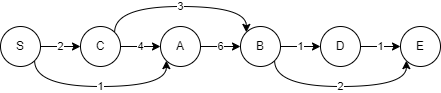
\includegraphics[scale=.6]{6_2_2_linearized_dag.png}
    \\Linearized DAG
  \end{center}
\end{quote}

I think we just need to initialize to $-\infty$ and update when we find a longer path.

\begin{algorithmic}
\State Initialize all $dist(\cdot)$ values to $-\infty$
\State $dist(s)=0$
\ForAll{$v\in{V\{s\}}$, in linearized order}
\State $dist(v)$=$max_{(u,v)\in{E}}\{dist(u)+l(u,v)\}$
\EndFor
\end{algorithmic}

\begin{center}
  \begin{tabular}{||c c c c c c c||}
    \hline
    Node & 0 & 1 & 2 & 3 & 4 & 5\\
    \hline\hline
    S & 0 & 0 & 0 & 0 & 0 & 0\\
    \hline
    C & $\infty$ & 2 & 2 & 2 & 2 & 2\\
    \hline
    A & $\infty$ & 1 & 6 & 6 & 6 & 6\\
    \hline
    B & $\infty$ & 5 & 5 & 10 & 10 & 10\\
    \hline
    D & $\infty$ & $\infty$ & $\infty$ & $\infty$ & 11 & 11\\
    \hline
    E & $\infty$ & $\infty$ & $\infty$ & 12 & 12 & 12\\
    \hline
  \end{tabular}
\end{center}

\end{document}